
\begingroup
\let\clearpage\relax
\chapter{FUNDAMENTAÇÃO TEÓRICA}\label{sec:fundamentacao}
\endgroup

A fundamentação teórica é uma parte essencial de qualquer trabalho acadêmico, pois fornece a base conceitual e teórica que sustenta a pesquisa. Alguns autores optam por intitular este capítulo como "Fundamentação Teórica", enquanto outros preferem "Revisão da Literatura". A escolha do título deve ser feita de acordo com a natureza do trabalho e a orientação do professor responsável. Recomenda-se consultar o orientador para definir o título mais adequado.

É importante evitar iniciar o capítulo diretamente com uma seção terciária. Sempre introduza o conteúdo com um texto explicativo que contextualize as seções subsequentes. Além disso, ao se referir a elementos específicos do trabalho, como capítulos, seções, figuras, tabelas ou equações, utilize a primeira letra maiúscula. Por exemplo, a Seção \ref{sec:citacoes} aborda as normas para citações bibliográficas. Observe no código-fonte deste documento como as referências cruzadas são feitas, permitindo a numeração automática e facilitando a inserção de novas seções.

\section{Inserindo Figuras}
\label{sec:figuras}

A inserção de figuras é uma prática comum em trabalhos acadêmicos para ilustrar conceitos, dados ou resultados. A Figura \ref{fig:reitoria} apresenta uma fotografia de exemplo. Ao inserir figuras, é importante seguir algumas diretrizes:

\begin{alineas}
    \item O título deve começar com a especificação do tipo de figura (fotografia, desenho, diagrama, fluxograma, gráfico, etc.). Utilize espaçamento simples (1 pt) e capitalize apenas a primeira letra da frase, exceto para nomes próprios. Não utilize ponto final no título.
   
    \item A largura da figura deve ser ajustada para preencher as margens da página, que possuem 16 cm de largura. Evite inserir figuras com menos de 7 cm de largura, pois podem comprometer a legibilidade.

    \item A figura deve ser posicionada o mais próximo possível do local onde foi mencionada no texto. Nunca insira uma figura antes de referenciá-la no texto.

    \item Sempre indique a fonte da figura. Caso a figura seja de autoria própria, utilize a expressão "Elaborado pelo autor".
\end{alineas}

\begin{figure}[h!] 
    \captionsetup{width=16cm} % Ajuste a largura do título para corresponder à figura
    \Caption{\label{fig:reitoria} Figura de Exemplo}
    \IFCEfig{}{
        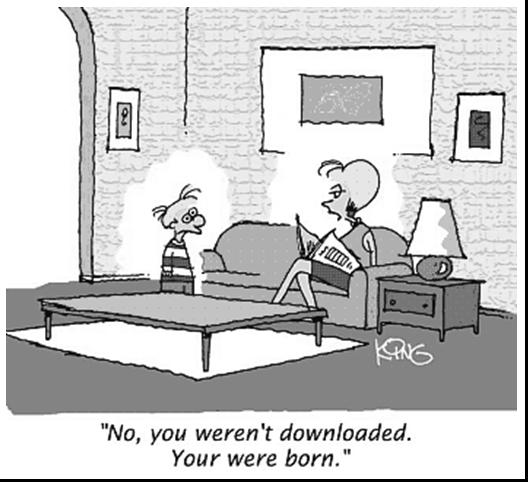
\includegraphics[width=16cm]{Figuras/fig1.jpg}
    }{
        \Fonte{Elaborado pelo Autor (2025)}
    }	
\end{figure}

Evite encerrar seções ou capítulos com figuras. Sempre adicione um texto explicativo após a figura para manter a fluidez do conteúdo.

\section{Inserindo Quadros}
\label{sec:quadros}

Quadros são utilizados para organizar informações de forma estruturada, especialmente quando se trata de dados qualitativos. O Quadro \ref{qua:exemplo-1} apresenta um exemplo de como inserir quadros no texto.

\begin{quadro}[h!]	
    \centering
    \Caption{\label{qua:exemplo-1} Exemplo de quadro com dados qualitativos}		
    \IFCEqua{}{
        \begin{tabular}{|c|c|l|l|}
            \hline
            Quisque & pharetra & tempus & vulputate \\
            \hline
            E1 & Complete coverage by a single transcript & Both  & Complete\\
            \hline
            E2 & Complete coverage by more than & Both splice sites & Complete\\
            \hline
            E3 & Partial coverage & Both splice sites & Both \\				
            \hline
        \end{tabular}
    }{
        \Fonte{Elaborado pelo autor.}
    }
\end{quadro}

\section{Inserindo Tabelas}
\label{sec:tabelas}

Tabelas são utilizadas para apresentar dados quantitativos organizadamente. A Tabela \ref{tab:exemplo-1} ilustra um exemplo de tabela alinhada. Ao inserir tabelas, siga as seguintes recomendações:

\begin{itemize}
    \item O título deve descrever o conteúdo da tabela de concisamente.
    \item Utilize linhas horizontais para separar os cabeçalhos dos dados. Evite o uso excessivo de linhas verticais.
    \item Sempre indique a fonte dos dados e inclua notas explicativas, se necessário.
\end{itemize}

\begin{table}[!h]
    \captionsetup{width=7cm} % Ajuste a largura do título para corresponder à tabela
    \Caption{\label{tab:exemplo-1} Exemplo de tabela com dados alinhados}
    \IBGEtab{}{%
        \begin{tabular}{ccc}
            \toprule
            Nome & Nascimento & Documento \\
            \midrule \midrule
            Maria da Silva & 11/11/1111 & 111.111.111-11 \\
            Maria da Silva & 11/11/1111 & 111.111.111-11 \\
            Maria da Silva & 11/11/1111 & 111.111.111-11 \\
            \bottomrule
        \end{tabular}%
    }{%
        \Fonte{O autor.}%
        \Nota{Esta é uma nota, que diz que os dados são baseados na regressão linear.}%
        \Nota[Anotações]{Uma anotação adicional, seguida de várias outras.}%
    }
\end{table}

\subsection{Exemplo de Subseção}
\label{sec:ex_sec}

Esta subseção serve como exemplo de como estruturar o conteúdo de forma hierárquica. Utilize subseções para dividir tópicos complexos em partes menores e mais gerenciáveis.

\section{Usando Fórmulas Matemáticas}
\label{sec:formulas}

Fórmulas matemáticas são frequentemente utilizadas em trabalhos acadêmicos para expressar relações quantitativas. Para inserir símbolos matemáticos no texto, utilize cifrões (\$). Por exemplo, $\alpha$, $\beta$ e $\gamma$ são símbolos do alfabeto grego. Para equações enumeradas, utilize o ambiente \texttt{equation}, como mostrado na Equação \ref{eq:indices}:

\begin{equation}
    \label{eq:indices}
    k_{n+1} = n^2 + k_n^2 - k_{n-1}.
\end{equation}

Observe que a equação faz parte da frase e deve ser pontuada corretamente. Ao referenciar a Equação \ref{eq:indices} no texto, utilize a primeira letra maiúscula.

Abaixo estão exemplos de equações com frações, matrizes e sistemas:

\begin{equation}
    \label{eq:fracao}
    \begin{aligned}
        x = a_0 + \cfrac{1}{a_1 + \cfrac{1}{a_2 + \cfrac{1}{a_3 + \cfrac{1}{a_4}}}}
    \end{aligned}.
\end{equation}

\begin{equation}
    \label{eq:matriz}
    \begin{aligned}
        A_{m,n} =
        \begin{pmatrix}
            a_{1,1} & a_{1,2} & \cdots & a_{1,n} \\
            a_{2,1} & a_{2,2} & \cdots & a_{2,n} \\
            \vdots  & \vdots  & \ddots & \vdots  \\
            a_{m,1} & a_{m,2} & \cdots & a_{m,n}
        \end{pmatrix}
    \end{aligned}.
\end{equation}

\begin{equation}
    \label{eq:sistema}
    \begin{aligned}
        f(n) = \left\{ 
        \begin{array}{l l}
            n/2 & \quad \text{se $n$ é par} \\
            -(n+1)/2 & \quad \text{se $n$ é ímpar}
        \end{array} \right.
    \end{aligned}.
\end{equation}
